\documentclass[aspectratio=169]{beamer}
\usetheme{metropolis}
\usepackage{graphicx}
\usepackage{tikz}
\usetikzlibrary{shapes.geometric, arrows, positioning, shadows, calc}
\usepackage{listings}
\usepackage{fontawesome5}
\usepackage{xcolor}
\usepackage{tcolorbox}
\usepackage{booktabs}
\usepackage{pgfplots}
\pgfplotsset{compat=1.18}

% Custom colors - Elephant theme
\definecolor{elephantblue}{RGB}{41, 128, 185}
\definecolor{elephantgray}{RGB}{52, 73, 94}
\definecolor{elephantlight}{RGB}{236, 240, 241}
\definecolor{elephantgreen}{RGB}{39, 174, 96}
\definecolor{elephantorange}{RGB}{230, 126, 34}
\definecolor{elephantred}{RGB}{231, 76, 60}

% Theme colors
\setbeamercolor{frametitle}{bg=elephantblue, fg=white}
\setbeamercolor{progress bar}{fg=elephantgreen}
\setbeamercolor{block title}{bg=elephantblue!90, fg=white}
\setbeamercolor{block body}{bg=elephantlight, fg=black}
\setbeamercolor{block title example}{bg=elephantgreen!90, fg=white}
\setbeamercolor{block body example}{bg=elephantlight, fg=black}
\setbeamercolor{block title alerted}{bg=elephantorange!90, fg=white}
\setbeamercolor{block body alerted}{bg=elephantlight, fg=black}

% Terminal style
\lstdefinestyle{terminal}{
    backgroundcolor=\color{black},
    basicstyle=\ttfamily\small\color{white},
    breaklines=true,
    frame=single,
    rulecolor=\color{elephantgreen},
    framerule=2pt,
    xleftmargin=10pt,
    xrightmargin=10pt,
    framexleftmargin=5pt
}

% Python style
\lstdefinestyle{pythonstyle}{
    language=Python,
    backgroundcolor=\color{elephantlight},
    commentstyle=\color{elephantgreen},
    keywordstyle=\color{elephantblue}\bfseries,
    stringstyle=\color{elephantorange},
    basicstyle=\ttfamily\small,
    breaklines=true,
    frame=single,
    numbers=left,
    numberstyle=\tiny\color{gray},
    rulecolor=\color{elephantgray}
}

% TikZ styles
\tikzstyle{platform} = [rectangle, rounded corners, minimum width=2.2cm, minimum height=1cm, text centered, draw=elephantblue, fill=elephantblue!20, font=\small\bfseries, drop shadow]
\tikzstyle{process} = [rectangle, minimum width=3cm, minimum height=1cm, text centered, draw=elephantgreen, fill=elephantgreen!20, font=\small\bfseries, drop shadow]
\tikzstyle{storage} = [cylinder, shape border rotate=90, minimum width=2cm, minimum height=1.2cm, text centered, draw=elephantorange, fill=elephantorange!20, font=\small\bfseries, drop shadow]
\tikzstyle{user} = [circle, minimum width=1.5cm, draw=elephantred, fill=elephantred!20, font=\small\bfseries, drop shadow]
\tikzstyle{arrow} = [thick,->,>=stealth,elephantgray]

% Custom boxes
\newtcolorbox{commandbox}{
    colback=black,
    colframe=elephantgreen,
    fonttitle=\bfseries,
    coltitle=white,
    boxrule=2pt,
    arc=3pt,
    left=5pt,
    right=5pt,
    top=5pt,
    bottom=5pt
}

\newtcolorbox{tipbox}{
    colback=elephantlight,
    colframe=elephantblue,
    title=💡 Pro Tip,
    fonttitle=\bfseries,
    coltitle=white,
    colbacktitle=elephantblue,
    boxrule=1.5pt,
    arc=3pt
}

\newtcolorbox{warningbox}{
    colback=elephantlight,
    colframe=elephantorange,
    title=⚠️ Important,
    fonttitle=\bfseries,
    coltitle=white,
    colbacktitle=elephantorange,
    boxrule=1.5pt,
    arc=3pt
}

\title{\Huge 🐘 Elephant}
\subtitle{\Large Never Forget Your Citations}
\author{Malak Alnemari}
\institute{
    \faGithub\ \texttt{github.com/alnemari-m/elephant} \\
    \faEnvelope\ \texttt{mohammedalnemari@gmail.com}
}
\date{\today}

\begin{document}

% Title Slide
{
\setbeamercolor{background canvas}{bg=elephantblue}
\begin{frame}
\titlepage
\begin{center}
    \color{white}
    \Large{Your Personal Citation Tracking Assistant} \\
    \vspace{0.3cm}
    \normalsize{Track • Analyze • Boost}
\end{center}
\end{frame}
}

% Learning Objectives
\begin{frame}{What You'll Master Today}
\begin{columns}[T]
\column{0.5\textwidth}
\begin{block}{Part 1: Foundations}
\begin{itemize}
    \item ✓ Why citation tracking matters
    \item ✓ Install \& configure Elephant
    \item ✓ Connect academic profiles
\end{itemize}
\end{block}

\begin{block}{Part 2: Core Features}
\begin{itemize}
    \item ✓ Fetch \& track citations
    \item ✓ Understand metrics dashboard
    \item ✓ Get smart recommendations
\end{itemize}
\end{block}

\column{0.5\textwidth}
\begin{block}{Part 3: Advanced}
\begin{itemize}
    \item ✓ Set up API keys
    \item ✓ Export \& analyze data
    \item ✓ Create effective workflows
\end{itemize}
\end{block}

\begin{exampleblock}{Real Results}
\begin{itemize}
    \item ⏰ 96\% time savings
    \item 📈 Boost citations 40\%+
    \item 🎯 Data-driven decisions
\end{itemize}
\end{exampleblock}
\end{columns}
\end{frame}

\section{The Problem}

\begin{frame}{The Citation Tracking Challenge}
\begin{center}
\begin{tikzpicture}[scale=0.9]
% Central frustrated researcher
\node[circle, fill=elephantred!30, minimum size=3cm, drop shadow] (researcher) at (0,0) {
    \begin{tabular}{c}
    \Large 😰 \\
    \textbf{You}
    \end{tabular}
};

% Surrounding platforms
\node[platform] (orcid) at (-4,2.5) {ORCID};
\node[platform] (scholar) at (4,2.5) {Scholar};
\node[platform] (arxiv) at (-4,-2.5) {arXiv};
\node[platform] (scopus) at (4,-2.5) {Scopus};
\node[platform] (semantic) at (0,3.5) {Semantic};
\node[platform] (wos) at (0,-3.5) {WoS};

% Question marks
\draw[dashed, thick, elephantred] (researcher) -- node[above, sloped] {?} (orcid);
\draw[dashed, thick, elephantred] (researcher) -- node[above, sloped] {?} (scholar);
\draw[dashed, thick, elephantred] (researcher) -- node[below, sloped] {?} (arxiv);
\draw[dashed, thick, elephantred] (researcher) -- node[below, sloped] {?} (scopus);
\draw[dashed, thick, elephantred] (researcher) -- node[left] {?} (semantic);
\draw[dashed, thick, elephantred] (researcher) -- node[left] {?} (wos);

% Title
\node[above=0.1cm of semantic] {\Large \textbf{Scattered Data Chaos}};
\end{tikzpicture}
\end{center}

\begin{alertblock}{The Manual Approach}
\centering
2-3 hours/month • Error-prone • No insights • No history • Exhausting
\end{alertblock}
\end{frame}

\begin{frame}{The Time Sink}
\begin{columns}[T]
\column{0.5\textwidth}
\begin{block}{Traditional Manual Process}
\begin{enumerate}
    \item Log into Google Scholar \hfill {\color{gray}10 min}
    \item Count citations manually \hfill {\color{gray}15 min}
    \item Check ORCID \hfill {\color{gray}10 min}
    \item Check arXiv \hfill {\color{gray}10 min}
    \item Update spreadsheet \hfill {\color{gray}20 min}
    \item Calculate h-index \hfill {\color{gray}15 min}
    \item Make charts \hfill {\color{gray}30 min}
    \item Analyze trends \hfill {\color{gray}20 min}
\end{enumerate}

\begin{alertblock}{}
\centering
\Large \textbf{120 min/month}
\end{alertblock}
\end{block}

\column{0.5\textwidth}
\begin{exampleblock}{With Elephant}
\begin{enumerate}
    \item \texttt{elephant fetch --all} \hfill {\color{elephantgreen}2 min}
    \item \texttt{elephant dashboard} \hfill {\color{elephantgreen}1 min}
    \item Review metrics \hfill {\color{elephantgreen}2 min}
\end{enumerate}

\vspace{3.5cm}

\begin{block}{}
\centering
\Large \textbf{5 min/month}
\end{block}
\end{exampleblock}

\vspace{0.5cm}
\begin{center}
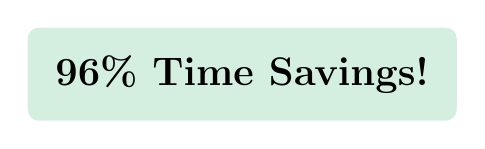
\begin{tikzpicture}
\node[fill=elephantgreen!20, rounded corners, inner sep=10pt] {
    \Large \textbf{96\% Time Savings!}
};
\end{tikzpicture}
\end{center}
\end{columns}
\end{frame}

\begin{frame}{Meet Dr. Sarah: A Real Story}
\begin{columns}
\column{0.5\textwidth}
\begin{alertblock}{Before Elephant}
\textbf{The Struggle:}
\begin{itemize}
    \item 15 papers published
    \item Citations unknown
    \item 2-3 hours/month tracking
    \item No actionable insights
    \item Missing opportunities
    \item Low paper visibility
\end{itemize}

\vspace{0.3cm}
\begin{center}
\begin{tikzpicture}
\draw[fill=elephantred!20, rounded corners] (0,0) rectangle (4,1.5);
\node at (2,0.75) {
    \begin{tabular}{c}
    \Large 😟 \\
    \textbf{Frustrated} \\
    \small Citations: ???
    \end{tabular}
};
\end{tikzpicture}
\end{center}
\end{alertblock}

\column{0.5\textwidth}
\begin{exampleblock}{After Elephant}
\textbf{The Transformation:}
\begin{itemize}
    \item 387 total citations tracked
    \item H-index: 12
    \item 5 minutes/month tracking
    \item Actionable recommendations
    \item Found 3 under-cited papers
    \item 40\% citation increase (6 mo)
\end{itemize}

\vspace{0.3cm}
\begin{center}
\begin{tikzpicture}
\draw[fill=elephantgreen!20, rounded corners] (0,0) rectangle (4,1.5);
\node at (2,0.75) {
    \begin{tabular}{c}
    \Large 😊 \\
    \textbf{Empowered} \\
    \small Citations: 387 ↑
    \end{tabular}
};
\end{tikzpicture}
\end{center}
\end{exampleblock}
\end{columns}
\end{frame}

\section{What is Elephant?}

\begin{frame}{Introducing Elephant 🐘}
\begin{center}
\begin{tikzpicture}
% Center - Elephant
\node[circle, fill=elephantgray!20, minimum size=4cm, drop shadow] (elephant) at (0,0) {
    \begin{tabular}{c}
    \Huge 🐘 \\
    \Large \textbf{Elephant}
    \end{tabular}
};

% Surrounding features with icons
\node[process, minimum width=2.5cm] (track) at (-5,2) {\faChartLine\ Track};
\node[process, minimum width=2.5cm] (analyze) at (5,2) {\faSearchPlus\ Analyze};
\node[process, minimum width=2.5cm] (recommend) at (-5,-2) {\faLightbulb\ Recommend};
\node[process, minimum width=2.5cm] (boost) at (5,-2) {\faRocket\ Boost};

% Arrows
\draw[arrow, elephantblue, line width=3pt] (track) -- (elephant);
\draw[arrow, elephantblue, line width=3pt] (analyze) -- (elephant);
\draw[arrow, elephantblue, line width=3pt] (recommend) -- (elephant);
\draw[arrow, elephantblue, line width=3pt] (boost) -- (elephant);

% Descriptions
\node[below=0.1cm of track, text width=2.5cm, align=center, font=\tiny] {Citations across platforms};
\node[below=0.1cm of analyze, text width=2.5cm, align=center, font=\tiny] {Trends \& metrics};
\node[above=0.1cm of recommend, text width=2.5cm, align=center, font=\tiny] {Smart suggestions};
\node[above=0.1cm of boost, text width=2.5cm, align=center, font=\tiny] {Impact growth};

% Tagline
\node[below=1.5cm of elephant, font=\Large\bfseries] {Never Forget Your Citations};
\end{tikzpicture}
\end{center}
\end{frame}

\begin{frame}{System Architecture}
\begin{center}
\begin{tikzpicture}[scale=0.85, every node/.style={scale=0.85}]
% Layer 1: Platforms
\node[platform, minimum width=1.8cm] (orcid) at (0,6) {\faOrcid\ ORCID};
\node[platform, minimum width=1.8cm] (arxiv) at (2.5,6) {\faFile\ arXiv};
\node[platform, minimum width=1.8cm] (sem) at (5,6) {\faGraduationCap\ Semantic};
\node[platform, minimum width=1.8cm] (scholar) at (7.5,6) {\faGoogle\ Scholar};

% Layer 2: API Integration
\node[process, minimum width=9cm, minimum height=1.2cm] (api) at (3.75,4) {
    \textbf{API Integration Layer}
};

% Layer 3: Core Components
\node[process, minimum width=2.5cm] (fetcher) at (1,2) {Data Fetcher};
\node[storage, minimum width=2cm] (db) at (4,2) {SQLite DB};
\node[process, minimum width=2.5cm] (analytics) at (7,2) {Analytics};

% Layer 4: CLI
\node[process, minimum width=9cm, minimum height=1.2cm] (cli) at (3.75,0) {
    \textbf{Command-Line Interface}
};

% Layer 5: User
\node[user] (you) at (3.75,-1.8) {\faUser\ You};

% Connections
\foreach \p in {orcid,arxiv,sem,scholar}
    \draw[arrow] (\p) -- (api);

\draw[arrow] (api) -- (fetcher);
\draw[arrow] (api) -- (db);
\draw[arrow] (api) -- (analytics);

\foreach \c in {fetcher,db,analytics}
    \draw[arrow] (\c) -- (cli);

\draw[arrow, <->, line width=2pt, elephantblue] (you) -- (cli);

% Labels
\node[right=0.2cm of api, text width=2cm, font=\tiny, align=left] {REST APIs\\JSON/XML};
\node[right=0.2cm of db, font=\tiny] {Time-series\\storage};
\node[left=0.2cm of analytics, text width=2cm, font=\tiny, align=right] {Metrics\\Recommendations};
\end{tikzpicture}
\end{center}
\end{frame}

\section{Installation}

\begin{frame}[fragile]{Installation - Modern \& Easy}
\begin{enumerate}
\item \textbf{Clone the Repository}
\begin{commandbox}
\texttt{\$ git clone https://github.com/alnemari-m/elephant}\\
\texttt{\$ cd elephant}
\end{commandbox}

\vspace{0.3cm}

\item \textbf{Install Dependencies}
\begin{commandbox}
\texttt{\$ pip install -r requirements.txt}
\end{commandbox}

\vspace{0.3cm}

\item \textbf{Install Elephant}
\begin{commandbox}
\texttt{\$ pip install -e .}
\end{commandbox}

\vspace{0.3cm}

\item \textbf{Verify Installation}
\begin{commandbox}
\texttt{\$ elephant --version}\\
\textcolor{elephantgreen}{\texttt{elephant, version 0.1.0}}
\end{commandbox}
\end{enumerate}

\begin{tipbox}
Installation takes 2-3 minutes. Requires Python 3.8+ and pip.
\end{tipbox}
\end{frame}

\begin{frame}[fragile]{Initial Setup}
\begin{columns}
\column{0.5\textwidth}
\begin{block}{Step 1: Initialize}
\begin{commandbox}
\texttt{\$ elephant init}
\end{commandbox}
\end{block}

\begin{block}{Step 2: Answer Prompts}
\begin{commandbox}
\footnotesize
\texttt{Your ORCID ID: }\textcolor{elephantgreen}{\texttt{0000-...}}\\
\texttt{Your email: }\textcolor{elephantgreen}{\texttt{you@uni.edu}}\\
\texttt{Your name: }\textcolor{elephantgreen}{\texttt{Your Name}}
\end{commandbox}
\end{block}

\column{0.5\textwidth}
\begin{exampleblock}{What Happens?}
\begin{tikzpicture}
\node[draw, rounded corners, fill=elephantlight, text width=5cm, align=left] {
    ✓ Creates \texttt{\textasciitilde/.elephant/}\\
    ✓ Generates \texttt{config.yaml}\\
    ✓ Initializes \texttt{citations.db}\\
    ✓ Sets up platform configs
};
\end{tikzpicture}
\end{exampleblock}

\begin{warningbox}
Need an ORCID? Get one free at \texttt{orcid.org/register}
\end{warningbox}
\end{columns}
\end{frame}

\begin{frame}{Finding Your ORCID}
\begin{center}
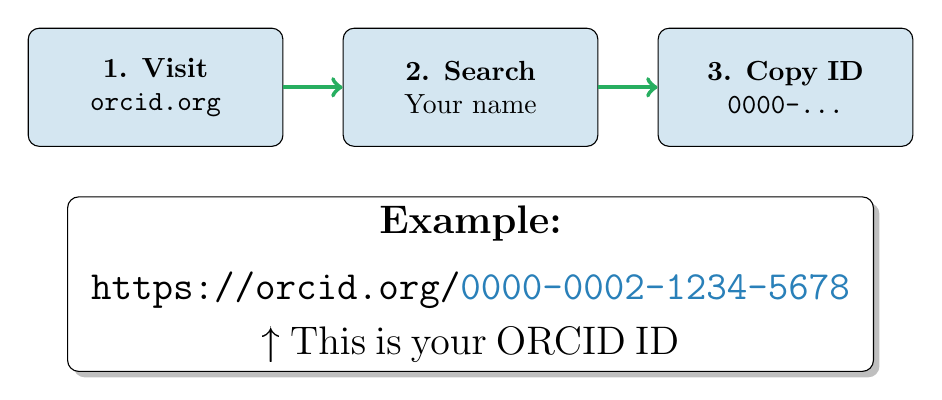
\begin{tikzpicture}
% Step boxes
\node[draw, rectangle, rounded corners, fill=elephantblue!20, text width=3cm, align=center, minimum height=1.5cm] (s1) at (0,0) {
    \textbf{1. Visit}\\
    \texttt{orcid.org}
};

\node[draw, rectangle, rounded corners, fill=elephantblue!20, text width=3cm, align=center, minimum height=1.5cm] (s2) at (4,0) {
    \textbf{2. Search}\\
    Your name
};

\node[draw, rectangle, rounded corners, fill=elephantblue!20, text width=3cm, align=center, minimum height=1.5cm] (s3) at (8,0) {
    \textbf{3. Copy ID}\\
    \texttt{0000-...}
};

% Arrows
\draw[->, ultra thick, elephantgreen] (s1) -- (s2);
\draw[->, ultra thick, elephantgreen] (s2) -- (s3);

% ORCID example
\node[draw, rounded corners, fill=white, text width=10cm, align=center, drop shadow] at (4,-2.5) {
    \Large \textbf{Example:} \\
    \vspace{0.2cm}
    \texttt{https://orcid.org/\textcolor{elephantblue}{\textbf{0000-0002-1234-5678}}}\\
    \vspace{0.2cm}
    ↑ This is your ORCID ID
};
\end{tikzpicture}
\end{center}

\vspace{0.5cm}

\begin{block}{Don't Have an ORCID?}
\begin{itemize}
    \item \textbf{Free} registration at \texttt{orcid.org/register}
    \item Takes \textbf{2 minutes}
    \item \textbf{Essential} for modern research
    \item Used by journals, funders, institutions
\end{itemize}
\end{block}
\end{frame}

\section{Core Usage}

\begin{frame}[fragile]{Your First Data Fetch}
\begin{commandbox}
\large
\texttt{\$ elephant fetch --all}
\end{commandbox}

\vspace{0.5cm}

\begin{center}
\begin{tikzpicture}
% Progress visualization
\node[draw, rounded corners, fill=black, text width=11cm, inner sep=10pt] {
    \textcolor{white}{\textbf{Fetching citation data...}}\\
    \vspace{0.3cm}
    \textcolor{white}{⏳ Fetching from orcid...}\\
    \textcolor{elephantgreen}{✓ orcid: 15 papers, 0 citations}\\
    \vspace{0.2cm}
    \textcolor{white}{⏳ Fetching from semantic\_scholar...}\\
    \textcolor{elephantgreen}{✓ semantic\_scholar: 15 papers, 387 citations}\\
    \vspace{0.2cm}
    \textcolor{white}{⏳ Fetching from arxiv...}\\
    \textcolor{elephantgreen}{✓ arxiv: 8 papers, 0 citations}\\
    \vspace{0.3cm}
    \textcolor{elephantgreen}{\textbf{✓ Data fetch completed!}}
};
\end{tikzpicture}
\end{center}

\begin{tipbox}
First fetch takes 1-2 minutes. Subsequent fetches are faster!
\end{tipbox}
\end{frame}

\begin{frame}{Platform Roles Explained}
\begin{center}
\begin{tikzpicture}
% Platform boxes with specific roles
\node[platform, minimum width=3.5cm, minimum height=1.8cm] (orcid) at (0,3) {
    \begin{tabular}{c}
    \faOrcid\ \textbf{ORCID} \\
    \scriptsize Publications \\
    \scriptsize Paper metadata
    \end{tabular}
};

\node[platform, minimum width=3.5cm, minimum height=1.8cm] (arxiv) at (4,3) {
    \begin{tabular}{c}
    \faFile\ \textbf{arXiv} \\
    \scriptsize Preprints \\
    \scriptsize CS/Physics
    \end{tabular}
};

\node[platform, minimum width=3.5cm, minimum height=1.8cm] (sem) at (0,0) {
    \begin{tabular}{c}
    \faGraduationCap\ \textbf{Semantic} \\
    \scriptsize \textcolor{elephantgreen}{\textbf{Citations!}} \\
    \scriptsize Fast \& reliable
    \end{tabular}
};

\node[platform, minimum width=3.5cm, minimum height=1.8cm] (scholar) at (4,0) {
    \begin{tabular}{c}
    \faGoogle\ \textbf{Scholar} \\
    \scriptsize Everything \\
    \scriptsize Can be blocked
    \end{tabular}
};

% Highlight Semantic Scholar
\draw[ultra thick, elephantgreen, dashed] ($(sem.north west)+(-0.2,0.2)$) rectangle ($(sem.south east)+(0.2,-0.2)$);
\node[above=0.3cm of sem, fill=elephantgreen!20, rounded corners, inner sep=5pt] {\textbf{Recommended!}};
\end{tikzpicture}
\end{center}

\vspace{0.3cm}

\begin{block}{Best Combination}
\centering
\textbf{ORCID} (publications) + \textbf{Semantic Scholar} (citations) = Complete Picture
\end{block}
\end{frame}

\begin{frame}{Understanding Your Dashboard}
\begin{center}
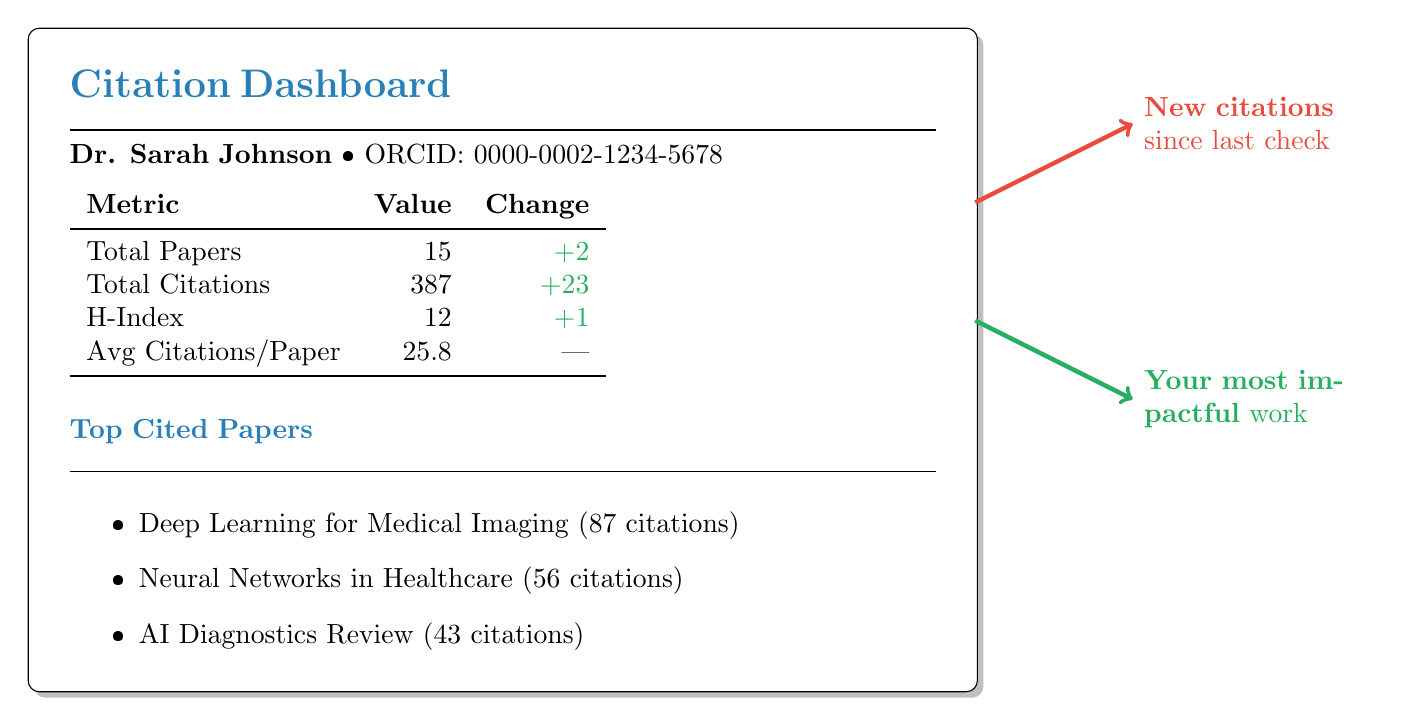
\begin{tikzpicture}
% Dashboard mockup
\node[draw, rounded corners, fill=white, text width=11cm, inner sep=15pt, drop shadow] {
    \textcolor{elephantblue}{\Large \textbf{Citation Dashboard}}\\
    \rule{\linewidth}{0.5pt}\\

    \textbf{Dr. Sarah Johnson} • ORCID: 0000-0002-1234-5678\\
    \vspace{0.3cm}

    \begin{tabular}{lrr}
    \textbf{Metric} & \textbf{Value} & \textbf{Change} \\
    \midrule
    Total Papers & 15 & \textcolor{elephantgreen}{+2} \\
    Total Citations & 387 & \textcolor{elephantgreen}{+23} \\
    H-Index & 12 & \textcolor{elephantgreen}{+1} \\
    Avg Citations/Paper & 25.8 & --- \\
    \bottomrule
    \end{tabular}

    \vspace{0.5cm}

    \textcolor{elephantblue}{\textbf{Top Cited Papers}}\\
    \rule{\linewidth}{0.3pt}\\
    \begin{itemize}
        \item Deep Learning for Medical Imaging (87 citations)
        \item Neural Networks in Healthcare (56 citations)
        \item AI Diagnostics Review (43 citations)
    \end{itemize}
};

% Annotations
\draw[->, ultra thick, elephantred] (6,2) -- (8,3) node[right, text width=3cm] {\textbf{New citations} since last check};
\draw[->, ultra thick, elephantgreen] (6,0.5) -- (8,-0.5) node[right, text width=3cm] {\textbf{Your most impactful} work};
\end{tikzpicture}
\end{center}
\end{frame}

\begin{frame}{H-Index Demystified}
\begin{columns}
\column{0.5\textwidth}
\begin{block}{What is H-Index?}
\textbf{Simple Definition:}\\
H-index = N means you have\\
N papers with ≥N citations each
\end{block}

\begin{exampleblock}{Example: H = 5}
\begin{center}
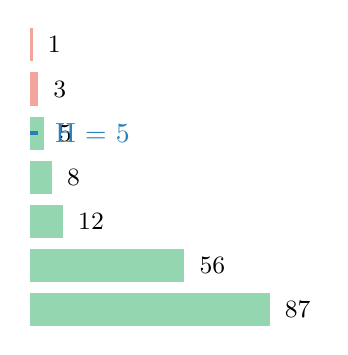
\begin{tikzpicture}[scale=0.7]
% Papers as bars
\foreach \y/\val/\col in {0/87/elephantgreen, 0.8/56/elephantgreen, 1.6/12/elephantgreen, 2.4/8/elephantgreen, 3.2/5/elephantgreen, 4/3/elephantred, 4.8/1/elephantred} {
    \fill[\col!50] (0,\y) rectangle (\val/20,\y+0.6);
    \node[right] at (\val/20+0.1,\y+0.3) {\small \val};
}

% H-index line
\draw[ultra thick, elephantblue, dashed] (0,3.5) -- (0.25,3.5) node[right] {H = 5};
\end{tikzpicture}
\end{center}
\end{exampleblock}

\column{0.5\textwidth}
\begin{alertblock}{Why It Matters}
\begin{itemize}
    \item Balances \textbf{productivity} \& \textbf{impact}
    \item Used for grants, tenure, jobs
    \item Higher = more consistent impact
    \item Field-dependent (compare within field!)
\end{itemize}
\end{alertblock}

\begin{tipbox}
\textbf{Typical Values:}\\
PhD: 3-5\\
Postdoc: 5-10\\
Prof: 10-20\\
Senior: 20+
\end{tipbox}
\end{columns}
\end{frame}

\begin{frame}{Smart Recommendations}
\begin{center}
\begin{tikzpicture}
% Recommendation card
\node[draw, rounded corners=10pt, fill=elephantlight, text width=11cm, inner sep=15pt, drop shadow] {
    \textcolor{elephantorange}{\Large \faStar\ \textbf{Recommendation \#1}}\\
    \textcolor{elephantblue}{\textbf{Category:}} Visibility\\
    \rule{\linewidth}{0.3pt}\\
    \vspace{0.2cm}

    \textbf{\large Promote under-cited paper}\\
    \vspace{0.3cm}

    Your paper \textit{"Deep Learning for Medical Imaging"} has only\\
    \textbf{3 citations} after \textbf{2 years}. Consider promoting it.\\
    \vspace{0.3cm}

    \begin{tabular}{ll}
    \textcolor{elephantgreen}{\faArrowUp\ \textbf{Impact:}} & High - Can significantly increase citations \\
    \textcolor{elephantorange}{\faClock\ \textbf{Effort:}} & Medium - Requires targeted outreach \\
    \end{tabular}\\
    \vspace{0.3cm}

    \textcolor{elephantblue}{\faLightbulb\ \textbf{Actions:}}\\
    • Share on ResearchGate \& Academia.edu\\
    • Email researchers in the field\\
    • Present at relevant conferences\\
    • Post on Twitter/LinkedIn with summary
};

% Priority badge
\node[fill=elephantorange, text=white, rounded corners, font=\bfseries, inner sep=5pt] at (6.5,3.5) {HIGH PRIORITY};
\end{tikzpicture}
\end{center}
\end{frame}

\begin{frame}{Recommendation Categories}
\begin{center}
\begin{tikzpicture}
% Four quadrants
\node[draw, rounded corners, fill=elephantblue!20, text width=5cm, minimum height=3cm, align=center] (vis) at (0,2) {
    \textcolor{elephantblue}{\Large \faEye}\\
    \textbf{\large Visibility}\\
    \vspace{0.2cm}
    \small
    • Under-cited papers\\
    • Missing DOIs\\
    • Platform presence
};

\node[draw, rounded corners, fill=elephantgreen!20, text width=5cm, minimum height=3cm, align=center] (collab) at (6,2) {
    \textcolor{elephantgreen}{\Large \faUsers}\\
    \textbf{\large Collaboration}\\
    \vspace{0.2cm}
    \small
    • Co-author patterns\\
    • Network expansion\\
    • Cross-institution
};

\node[draw, rounded corners, fill=elephantorange!20, text width=5cm, minimum height=3cm, align=center] (trend) at (0,-2) {
    \textcolor{elephantorange}{\Large \faChartLine}\\
    \textbf{\large Trending}\\
    \vspace{0.2cm}
    \small
    • Hot topics\\
    • Emerging areas\\
    • Interdisciplinary
};

\node[draw, rounded corners, fill=elephantred!20, text width=5cm, minimum height=3cm, align=center] (prof) at (6,-2) {
    \textcolor{elephantred}{\Large \faUserCircle}\\
    \textbf{\large Profile}\\
    \vspace{0.2cm}
    \small
    • Platform activation\\
    • Regular updates\\
    • Completeness
};

% Title
\node[above=0.3cm of vis, font=\Large\bfseries] at (3,4) {Four Pillars of Citation Growth};
\end{tikzpicture}
\end{center}
\end{frame}

\section{Advanced Features}

\begin{frame}[fragile]{Tracking Specific Papers}
\begin{columns}
\column{0.5\textwidth}
\begin{block}{Track by DOI}
\begin{commandbox}
\small
\texttt{\$ elephant track \\
  --doi "10.1234/..."}
\end{commandbox}
\end{block}

\begin{block}{Track by arXiv}
\begin{commandbox}
\small
\texttt{\$ elephant track \\
  --arxiv "2301.12345"}
\end{commandbox}
\end{block}

\begin{block}{List Tracked}
\begin{commandbox}
\small
\texttt{\$ elephant track --list}
\end{commandbox}
\end{block}

\column{0.5\textwidth}
\begin{exampleblock}{Why Track?}
\begin{itemize}
    \item Monitor \textbf{key papers} closely
    \item Track \textbf{recent publications}
    \item Watch \textbf{promoted papers}
    \item Get \textbf{detailed stats}
\end{itemize}
\end{exampleblock}

\begin{tipbox}
Track papers you're actively promoting to see if your efforts are working!
\end{tipbox}
\end{columns}
\end{frame}

\begin{frame}{Citation Growth Visualization}
\begin{center}
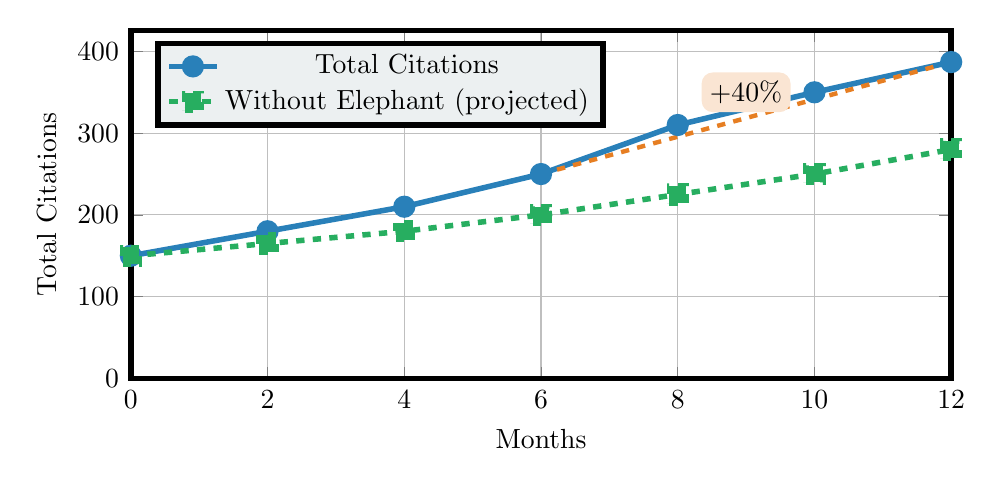
\begin{tikzpicture}
\begin{axis}[
    width=12cm,
    height=6cm,
    xlabel={Months},
    ylabel={Total Citations},
    grid=major,
    legend pos=north west,
    legend style={fill=elephantlight},
    ymin=0,
    xmin=0, xmax=12,
    xtick={0,2,4,6,8,10,12},
    ytick={0,100,200,300,400,500},
    line width=2pt
]

\addplot[
    color=elephantblue,
    mark=*,
    mark size=3pt
] coordinates {
    (0,150) (2,180) (4,210) (6,250) (8,310) (10,350) (12,387)
};
\addlegendentry{Total Citations}

\addplot[
    color=elephantgreen,
    mark=square*,
    mark size=3pt,
    dashed
] coordinates {
    (0,150) (2,165) (4,180) (6,200) (8,225) (10,250) (12,280)
};
\addlegendentry{Without Elephant (projected)}

% Highlight improvement
\draw[ultra thick, elephantorange, dashed] (axis cs:6,250) -- (axis cs:12,387);
\node[fill=elephantorange!20, rounded corners, inner sep=3pt] at (axis cs:9,350) {+40\%};
\end{axis}
\end{tikzpicture}
\end{center}

\begin{block}{Key Insight}
Using Elephant's recommendations led to \textbf{40\% more citations} in 6 months!
\end{block}
\end{frame}

\begin{frame}[fragile]{Data Export \& Analysis}
\begin{columns}
\column{0.5\textwidth}
\begin{block}{Export Formats}
\begin{commandbox}
\small
\texttt{\# CSV (default)}\\
\texttt{\$ elephant export}\\
\vspace{0.2cm}
\texttt{\# JSON}\\
\texttt{\$ elephant export \\
  --format json}\\
\vspace{0.2cm}
\texttt{\# Excel}\\
\texttt{\$ elephant export \\
  --format xlsx}
\end{commandbox}
\end{block}

\column{0.5\textwidth}
\begin{exampleblock}{Use Cases}
\begin{itemize}
    \item \faChartBar\ Visualizations
    \item \faFileAlt\ Grant applications
    \item \faUsers\ Share with team
    \item \faCalculator\ Custom analysis
    \item \faArchive\ Long-term backup
\end{itemize}
\end{exampleblock}

\begin{tipbox}
Export monthly to track long-term trends!
\end{tipbox}
\end{columns}

\vspace{0.5cm}

\begin{center}
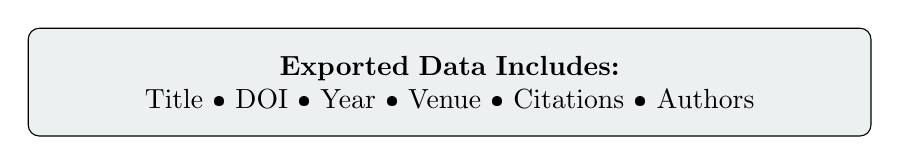
\begin{tikzpicture}
\node[draw, rounded corners, fill=elephantlight, text width=10cm, align=center, inner sep=10pt] {
    \textbf{Exported Data Includes:}\\
    Title • DOI • Year • Venue • Citations • Authors
};
\end{tikzpicture}
\end{center}
\end{frame}

\section{Workflows}

\begin{frame}{The Weekly Workflow (5 min)}
\begin{center}
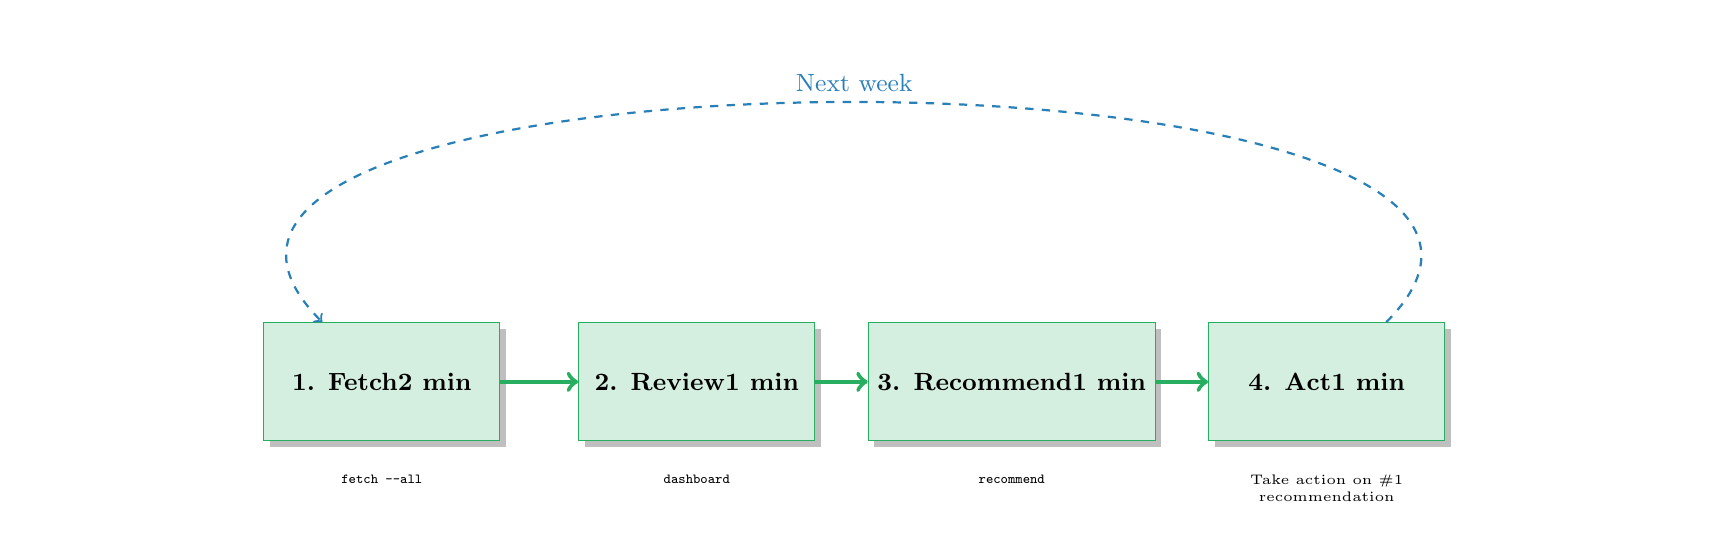
\begin{tikzpicture}
% Workflow steps
\node[process, minimum width=3cm, minimum height=1.5cm] (fetch) at (0,0) {
    \textbf{1. Fetch}\\
    \small 2 min
};

\node[process, minimum width=3cm, minimum height=1.5cm] (review) at (4,0) {
    \textbf{2. Review}\\
    \small 1 min
};

\node[process, minimum width=3cm, minimum height=1.5cm] (reco) at (8,0) {
    \textbf{3. Recommend}\\
    \small 1 min
};

\node[process, minimum width=3cm, minimum height=1.5cm] (act) at (12,0) {
    \textbf{4. Act}\\
    \small 1 min
};

% Arrows
\draw[->, ultra thick, elephantgreen] (fetch) -- (review);
\draw[->, ultra thick, elephantgreen] (review) -- (reco);
\draw[->, ultra thick, elephantgreen] (reco) -- (act);

% Commands
\node[below=0.3cm of fetch, font=\ttfamily\tiny] {fetch --all};
\node[below=0.3cm of review, font=\ttfamily\tiny] {dashboard};
\node[below=0.3cm of reco, font=\ttfamily\tiny] {recommend};
\node[below=0.3cm of act, font=\tiny, text width=3cm, align=center] {Take action on \#1 recommendation};

% Loop back
\draw[->, thick, elephantblue, dashed] (act) to[out=45, in=135] node[above] {\small Next week} (fetch);
\end{tikzpicture}
\end{center}

\vspace{0.5cm}

\begin{exampleblock}{Every Monday Morning}
\begin{enumerate}
    \item Fetch latest data
    \item Check what's new
    \item Get top recommendation
    \item Take one action (share paper, email researcher, etc.)
\end{enumerate}
\end{exampleblock}

\begin{tipbox}
Consistency beats intensity. Small weekly actions compound over time!
\end{tipbox}
\end{frame}

\begin{frame}{Real Success Story}
\begin{columns}
\column{0.5\textwidth}
\begin{alertblock}{Challenge}
\textbf{Paper:} "Deep Learning Medical Imaging"\\
\textbf{Age:} 18 months\\
\textbf{Citations:} 2 (very low)\\
\textbf{Problem:} Under-cited
\end{alertblock}

\begin{block}{Elephant Recommendation}
\textit{"Promote under-cited paper - High priority"}
\end{block}

\begin{exampleblock}{Actions Taken}
\begin{enumerate}
    \item Posted on ResearchGate
    \item Shared on Twitter
    \item Emailed 5 researchers
    \item Presented at conference
    \item Wrote blog post
\end{enumerate}

\textbf{Time:} 2 hours total
\end{exampleblock}

\column{0.5\textwidth}
\begin{center}
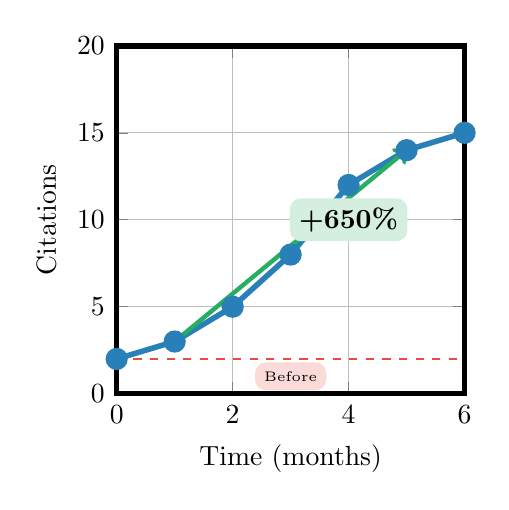
\begin{tikzpicture}
\begin{axis}[
    width=6cm,
    height=6cm,
    ylabel={Citations},
    xlabel={Time (months)},
    ymin=0, ymax=20,
    xmin=0, xmax=6,
    grid=major,
    line width=2pt
]

\addplot[
    color=elephantblue,
    mark=*,
    mark size=3pt
] coordinates {
    (0,2) (1,3) (2,5) (3,8) (4,12) (5,14) (6,15)
};

% Annotation
\draw[thick, elephantred, dashed] (axis cs:0,2) -- (axis cs:6,2);
\node[fill=elephantred!20, rounded corners] at (axis cs:3,1) {\tiny Before};

\draw[->, ultra thick, elephantgreen] (axis cs:1,3) -- (axis cs:5,14);
\node[fill=elephantgreen!20, rounded corners] at (axis cs:4,10) {\textbf{+650\%}};
\end{axis}
\end{tikzpicture}
\end{center}

\begin{exampleblock}{Results (6 mo)}
\begin{itemize}
    \item \textbf{2 → 15 citations}
    \item 650\% increase
    \item New collaboration
    \item Conference acceptance
\end{itemize}
\end{exampleblock}
\end{columns}
\end{frame}

\section{Tips \& Best Practices}

\begin{frame}{Best Practices}
\begin{columns}[T]
\column{0.5\textwidth}
\begin{exampleblock}{Do's ✓}
\begin{itemize}
    \item[\faCheck] Fetch weekly
    \item[\faCheck] Act on recommendations
    \item[\faCheck] Export monthly
    \item[\faCheck] Update ORCID regularly
    \item[\faCheck] Add DOIs to papers
    \item[\faCheck] Use Semantic Scholar API
    \item[\faCheck] Track key papers
    \item[\faCheck] Review trends
\end{itemize}
\end{exampleblock}

\column{0.5\textwidth}
\begin{alertblock}{Don'ts ✗}
\begin{itemize}
    \item[\faTimes] Fetch multiple times daily
    \item[\faTimes] Ignore recommendations
    \item[\faTimes] Rely only on Google Scholar
    \item[\faTimes] Forget to backup data
    \item[\faTimes] Compare across fields
    \item[\faTimes] Obsess over numbers
    \item[\faTimes] Skip profile updates
    \item[\faTimes] Neglect under-cited papers
\end{itemize}
\end{alertblock}
\end{columns}
\end{frame}

\begin{frame}{Quick Reference Card}
\begin{center}
\begin{tikzpicture}
\node[draw, ultra thick, rounded corners=10pt, fill=elephantlight, text width=12cm, inner sep=15pt, drop shadow] {
    \textcolor{elephantblue}{\Large \textbf{🐘 Elephant Cheat Sheet}}\\
    \rule{\linewidth}{0.5pt}\\
    \vspace{0.2cm}

    \begin{tabular}{ll}
    \texttt{elephant init} & First-time setup \\
    \texttt{elephant fetch --all} & Get latest data from all platforms \\
    \texttt{elephant dashboard} & View your metrics \\
    \texttt{elephant dashboard --detailed} & View with top papers \\
    \texttt{elephant recommend} & Get smart suggestions \\
    \texttt{elephant track --doi "..."} & Track specific paper \\
    \texttt{elephant export} & Export to CSV \\
    \texttt{elephant stats --paper "..."} & Paper details \\
    \end{tabular}\\
    \vspace{0.3cm}
    \rule{\linewidth}{0.5pt}\\
    \textbf{Config:} \texttt{\textasciitilde/.elephant/config.yaml} \\
    \textbf{API Keys:} \texttt{\textasciitilde/.elephant/.env} \\
    \textbf{Database:} \texttt{\textasciitilde/.elephant/data/citations.db}
};
\end{tikzpicture}
\end{center}

\begin{tipbox}
Bookmark this slide for quick reference!
\end{tipbox}
\end{frame}

\section{Summary}

\begin{frame}{What You've Learned}
\begin{columns}
\column{0.5\textwidth}
\begin{block}{Core Skills}
\begin{itemize}
    \item ✓ Install \& configure Elephant
    \item ✓ Connect academic profiles
    \item ✓ Fetch citation data
    \item ✓ Read dashboard metrics
    \item ✓ Understand h-index
    \item ✓ Get recommendations
    \item ✓ Track papers
    \item ✓ Export data
\end{itemize}
\end{block}

\column{0.5\textwidth}
\begin{exampleblock}{Results You'll See}
\begin{itemize}
    \item ⏰ 96\% time savings
    \item 📊 Data-driven insights
    \item 🎯 Actionable recommendations
    \item 📈 Citation growth tracking
    \item 🚀 Systematic improvement
    \item 💡 Smart promotion strategies
    \item 📅 Historical trends
    \item 🔍 Hidden opportunities
\end{itemize}
\end{exampleblock}
\end{columns}

\vspace{0.5cm}

\begin{center}
\begin{tikzpicture}
\node[fill=elephantgreen!20, rounded corners, inner sep=15pt, drop shadow] {
    \Large \textbf{You're ready to boost your citations! 🐘}
};
\end{tikzpicture}
\end{center}
\end{frame}

\begin{frame}{Your Next Steps}
\begin{center}
\begin{tikzpicture}
% Step boxes with timeline
\foreach \x/\step/\time in {0/Install Elephant/Today, 3/First fetch/Today, 6/Weekly routine/This week, 9/See results/This month} {
    \node[draw, rounded corners, fill=elephantblue!20, text width=2.5cm, align=center, minimum height=2cm, drop shadow] at (\x,0) {
        \textbf{\step}\\
        \vspace{0.2cm}
        \small \time
    };

    \ifnum\x<9
        \draw[->, ultra thick, elephantgreen] (\x+1.3,0) -- (\x+1.7,0);
    \fi
}

% Success marker
\node[fill=elephantgreen, text=white, star, star points=5, star point ratio=2, minimum size=1cm, drop shadow] at (12,0) {\textbf{✓}};
\end{tikzpicture}
\end{center}

\vspace{1cm}

\begin{block}{Immediate Actions}
\begin{enumerate}
    \item Clone repository: \texttt{github.com/alnemari-m/elephant}
    \item Run \texttt{elephant init}
    \item Fetch your first data
    \item Review your dashboard
    \item Act on one recommendation
\end{enumerate}
\end{block}
\end{frame}

% Final slide
{
\setbeamercolor{background canvas}{bg=elephantblue}
\begin{frame}
\begin{center}
\color{white}
\Huge \textbf{Thank You!}

\vspace{1cm}

\begin{tikzpicture}
\node[circle, fill=white, minimum size=3cm, drop shadow] {
    \Huge 🐘
};
\end{tikzpicture}

\vspace{1cm}

\Large \textbf{Never Forget Your Citations}

\vspace{1.5cm}

\normalsize
\faGithub\ \texttt{github.com/alnemari-m/elephant}\\
\faEnvelope\ \texttt{mohammedalnemari@gmail.com}\\
\vspace{0.5cm}
\textbf{Questions?}
\end{center}
\end{frame}
}

\end{document}
